\documentclass[12pt, a4paper]{article}

% Ru lang stuff
\usepackage [utf8x] {inputenc}
\usepackage [T2A] {fontenc}

% running titles 
\usepackage{fancybox}
\usepackage{fancyhdr}

% for last page number
\usepackage{lastpage}

%for colored tablets cells
\usepackage{colortbl}

% for Ru text in formulas
\usepackage[warn]{mathtext}

% for captions 
\usepackage[labelsep=period]{caption}
\usepackage{capt-of}

% for colored hyperrefs
\usepackage{xcolor}
\usepackage{hyperref}

% for pictures 
\usepackage{graphicx}

% for coll math
\usepackage{amsmath}

% path to all pictures
\graphicspath{{picks/}}

% for enumerates
\usepackage[shortlabels]{enumitem}

% for diff running titles on pages with diff parity
\usepackage{ifthen}
\usepackage{pdfpages}
\usepackage[strict]{changepage}

% for graphics
\usepackage{pgfplots}
\pgfplotsset{compat=1.9}

%for drawings
\usepackage{tikz}
\usetikzlibrary{calc}
\usetikzlibrary{decorations.pathmorphing}

% for good text in tablets
\usepackage{array}

% upgrading tables
\newcolumntype{P}[1]{>{\centering\arraybackslash}p{#1}}
\newcolumntype{M}[1]{>{\centering\arraybackslash}m{#1}}


% dock fields 20 15 15 35
\usepackage[left=12mm, top=12mm, right=15mm, bottom=28mm, nohead, footskip=10mm]{geometry}

% for cool tables
\usepackage{multirow}

% for different section/subsection/subsubsection styles in contents and doc
\usepackage[english, russian]{babel}

\usepackage{amsmath}

% for cool tables
\usepackage{tabularx}

\newcommand{\sect}[2] {
    \addtocounter{section}{1}
    \section*{\Huge\thesection.\,#1}
    \addcontentsline{toc}{subsection}{ \texorpdfstring{\thesection.\qquad\qquad #2}{Lg}}
}

\newcommand{\subsec}[2] {
    \addtocounter{subsection}{1}
    \subsection*{\thesubsection.\,#1}
    \addcontentsline{toc}{subsection}{ \texorpdfstring{\quad \thesubsection.\qquad\ #2}{Lg}}
}

\newcommand{\subsubsec}[2] {
    \addtocounter{subsubsection}{1}
    \subsubsection*{\thesubsubsection.\,#1}
    \addcontentsline{toc}{subsection}{ \texorpdfstring{\quad\quad\ \thesubsubsection. #2}{Lg}}
}
%-------------------------------------------------------------------------%

% for easy mini pages with shifts
\newcommand{\shiftedText}[3]{
\hspace*{#1}\begin{minipage}[t]{#2}
#3
\end{minipage}
}

\newcolumntype{P}[1]{>{\centering\arraybackslash}p{#1}}

% page style setup (for running titles)
\fancypagestyle{plain}{ %
\fancyhf{} % remove everything

 % lines parameters
\renewcommand{\headrulewidth}{0pt}
\renewcommand{\footrulewidth}{0pt}

% running titles contents
\fancyfoot[L]{\ifthenelse{\isodd{\thepage}}{Работа 1.3.1}{\thepage}}
\fancyfoot[R]{\ifthenelse{\isodd{\thepage}}{\thepage}{Работа 1.3.1}}
}

% choosing page style with our running titles
\pagestyle{plain}

\tolerance = 10000

\title{Лабораторная работа №1.3.1}
\author{Mikhail Pavlov \thanks{MIPT}}
\date{December, 2021}
\begin{document}


\shiftedText{0.5cm}{14cm}
{
    \begin{center}
    \vspace*{1.0cm}    
        
        {\bf\Huge Работа 1.3.1 }
        
    \vspace*{0.2cm}    
        
        {\bf\LARGE Определение модуля Юнга по измерениям растяжения проволоки. }
        
    \vspace*{0.8cm}
        {\LARGE Работу выполнил Павлов Михаил Б01-109 }
        
    \vspace*{1.6cm}
    
    \end{center}
}

\fancypagestyle{plain}{ %
\fancyhf{} % remove everything

 % lines parameters
\renewcommand{\headrulewidth}{0pt}
\renewcommand{\footrulewidth}{0pt}
% running titles contents
\fancyfoot[L]{\ifthenelse{\isodd{\thepage}}{Работа 1.3.1}{\thepage}}
\fancyfoot[R]{\ifthenelse{\isodd{\thepage}}{\thepage}{Работа 1.3.1}}
}

% choosing page style with our running titles
\pagestyle{plain}

\tolerance = 10000

\vspace*{0.6cm}

{\Large 1. Аннотация \\}

В данной работе с помощью прибора Лермантова и проволоки экспериментально 
доказывается зависимость между напряжением и деформацией проволоки, а также рассчитывается модуль Юнга и
сравнивается с табличным значением.

\vspace{1cm}
{\Large 2. Теоретические сведения \\}

Основное уравнение для описания одноосного напряженного состояния: 

\begin{equation}
    \varsigma = E\varepsilon
\end{equation}
где $\varepsilon$ --- деформация в точке, $E$ --- модуль Юнга, а $\varsigma$ --- напряжение.

\vspace{1cm}
{\Large 3. Инструментальные погрешности \\}
\noindent
\textbf{Рулетка: } $\sigma_{rul} = \pm 0.5$ мм (половина цены деления)\\
\textbf{Микрометр: } $\sigma_{mic} = \pm 0.01$ мм (маркировка производителя) \\
\textbf{Шкала: } $\sigma_{sc} = \pm 0.1$ см (маркировка производителя) \\

\newpage
{\Large 4. Экспериментальная установка \\}

Для определения модуля Юнга используется прибор Лермантова, изображенный на рис. 1.


\noindent\begin{minipage}[c]{0.53\textwidth}
    \hspace{1cm}
    Верхний конец проволоки П, изготовленной из ислледуемого материала, прикреплен к консоли К,
    а нижний --- к цилиндру, которым оканчивается шарнирный кронштейн Ш. На этот же цилиндр опирается рычаг $r$, связанный
    с зеркальцем З. Таким образом, удлинение проволоки можно измерить по углу поворота зеркальца.

    Натяжение проволоки можно менять, перекладывая грузы с площадки М на площадку О и наоборот.
    Такая система позволяет исключить влияние деформации кронштейна К на точность измерений,
    так как нагрузка на нем все время остается постоянной.

    Стоит отметить, что при отсутствии нагрузки проволока П всегда несколько изогнута, поэтому 
    вначале она не столько растягивается, сколько распрямляется.

\end{minipage}
\begin{minipage}[c]{0.42\textwidth}
    \begin{center}
        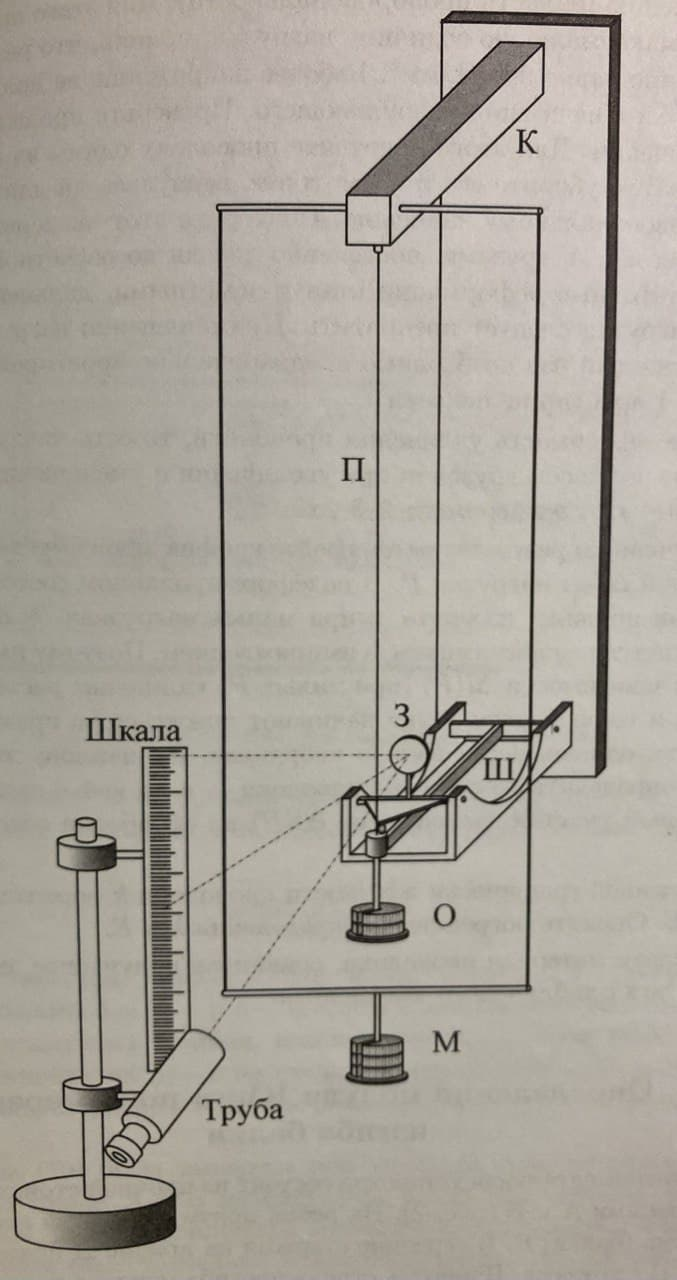
\includegraphics[scale=0.3]{Pics/Picture1.jpg} \\
        \textit{\textcolor[HTML]{000000}{Рис. 1. Прибор Лермантова}}
    \end{center}
\end{minipage}  


\vspace*{0.3cm}
{\Large 5. Результаты измерений и обработка данных \\} 

\begin{enumerate}
    \item $d = (0,46 \pm 0,01) \text{мм}$.
    \item Измеряем площадь поперечного сечения проволоки
    \[S =\dfrac{ \pi (\overline{d})^2}{4} = 0,166 \text{ мм}^2\]
    \[\sigma_S = S\sqrt{2\left( \dfrac{\sigma_d}{d}\right) ^2} = 0,005 \text{ мм}^2\]
    \[S = (0,166\pm0,005) \text{ мм}^2\]
    \item Измеряем длинну проволоки $l = 176,5  \text{ см}$
    \item Направляем зрительную трубу на зеркальце так, чтобы мы четко видели шкалу, тогда свет от шкалы будет падать примерно перпендикулярно шкале на зеркало, поэтому
    \[\Delta l =\dfrac{nr}{2h}\]
    \[ \sigma_{\Delta l} = \Delta l\sqrt{\left( \dfrac{\sigma_{n}}{n}\right)^2 + \left(\dfrac{\sigma_d}{d}\right)^2+\left(\dfrac{\sigma_h}{h}\right)^2} \]
    где $r = 15$ см - длина рычага, разница показаний шкалы - $n$, расстояние от шкалы до проволоки - $h = (134,5\pm0,1)\text{ см}$.
    \item Занесем полученные данные в таблицу 
    
    \begin{table}
        \center{
        \begin{tabular}{|c|c|c|c|c|c||c|c|c|c|c|}
        \hline
        P, Н & 9,48 &14,41 &18,87&23,60 &28,53 &28,53 &23,60 &18,87 &14,41 &9,48\\
        \hline
        $\Delta l$, см&0,326 &0,641 &0,897 &1,168 &1,440 &1,440 &1,163 &0,902 &0,641 &0,342\\ 
        \hline
        $\sigma_{\Delta l}$&0,007 &0,014 &0,020 &0,025 &0,031 &0,031 &0,025 &0,020 &0,014 &0,008\\
        \hline
        \hline
        P, Н & 9,48 &14,41 &18,87&23,60 &28,53 &28,53 &23,60 &18,87 &14,41 &9,48\\
        \hline
        $\Delta l$, см&0,331 &0,630 &0,886 &1,152 &1,429 &1,429 &1,152 &0,886 &0,630 &0,326\\
        \hline
        $\sigma_{\Delta l}$&0,007 &0,014 &0,019 &0,025 &0,031 &0,031 &0,025 &0,019 &0,014 &0,007\\
        \hline
        \hline
        P, Н & 9,48 &14,41 &18,87&23,60 &28,53 &28,53 &23,60 &18,87 &14,41 &9,48\\
        \hline
        $\Delta l$&0,315 &0,630 &0,880 &1,158 &1,429 &1,424 &1,152 &0,870 &0,614 &0,337\\
        \hline
        $\sigma_{\Delta l}$&0,007 &0,014 &0,019 &0,025 &0,031 &0,031 &0,025 &0,019 &0,013 &0,008\\
        \hline
        \end{tabular}
        }
        \caption{Зависимость удлинения проволоки от нагрузки}
    \end{table}

    \item Построим график зависимости удлинения проволоки от нагрузки. Найдем уравнение получившийся прямой по МНК. По наклону прямой определим жесткость проволоки, а по ней --- модуль Юнга. 
    
    \begin{tikzpicture}
        \begin{axis} [title = Рис. 2. Зависимость удлинения проволоки от нагрузки,
                xlabel=$\Delta l \text{, мм}$,
                ylabel= {P, Н}]
        \addplot coordinates {
        (0.84, 2.40)
        (0.99, 4.81)
        (1.13, 7.20)
        (1.27, 9.60)
        (1.41, 12.02)
        (1.54, 14.42)
        (1.67, 16.83)
        (1.81, 19.24)
        (1.94, 21.64)
        };
        \addplot coordinates {
        (0.84, 2.40)
        (1.94, 21.34)
        };
        \end{axis}
        \end{tikzpicture}

        Отсюда находим $k = 1.72 \cdot 10^3 \pm 0.027 \cdot 10^3$ Н/м.

    \item Наконец, по найденной графически жёсткости проволоки найдем модуль Юнга по формуле
    \[E = \dfrac{k*l_0}{S}\]
    \[\sigma_E = \sqrt{\left( \dfrac{\sigma_{k}}{k} \right)^2 + \left( \dfrac{\sigma_{S}}{S} \right)^2 + \left( \dfrac{\sigma_{l_0}}{l_0} \right)^2 }\]
    \end{enumerate}   

    \underline{Окончательный результат:} E = $18.4 \pm 0.7 \cdot 10^{10}$ Па \\ 


\end{document}